%%%%%%%%%%%%%%%%%%%%%%%%%%%%%%%%%%%%%%%%%%%%%%%%%%%%%%%%%%%%%%%
%
% Welcome to Overleaf --- just edit your LaTeX on the left,
% and we'll compile it for you on the right. If you open the
% 'Share' menu, you can invite other users to edit at the same
% time. See www.overleaf.com/learn for more info. Enjoy!
%
%%%%%%%%%%%%%%%%%%%%%%%%%%%%%%%%%%%%%%%%%%%%%%%%%%%%%%%%%%%%%%%


% Inbuilt themes in beamer
\documentclass{beamer}

% Theme choice:
\usetheme{CambridgeUS}

% Packages
\usepackage{graphicx}
\graphicspath{{images/}}
\usepackage{gensymb}
\usepackage{amssymb}
\usepackage[cmex10]{amsmath}
\usepackage{amsthm}
\usepackage[export]{adjustbox}
\usepackage{bm}
\usepackage{longtable}
\usepackage{enumitem}
\usepackage{mathtools}
 \usepackage{tikz}
\usepackage[breaklinks=true]{hyperref}
\usepackage{listings}
\usepackage{color}                                            %%
\usepackage{array}                                            %%
\usepackage{longtable}                                        %%
\usepackage{calc}                                             %%
\usepackage{multirow}                                         %%
\usepackage{hhline}                                           %%
\usepackage{ifthen}                                           %%
\usepackage{lscape}     
\usepackage{multicol}
\usepackage{enumerate}
\DeclareMathOperator*{\Res}{Res}
\renewcommand\thesection{\arabic{section}}
\renewcommand\thesubsection{\thesection.\arabic{subsection}}
\renewcommand\thesubsubsection{\thesubsection.\arabic{subsubsection}}
\renewcommand\thesectiondis{\arabic{section}}
\renewcommand\thesubsectiondis{\thesectiondis.\arabic{subsection}}
\renewcommand\thesubsubsectiondis{\thesubsectiondis.\arabic{subsubsection}}
\hyphenation{op-tical net-works semi-conduc-tor}
\def\inputGnumericTable{}                                 %%
\lstset{
frame=single, 
breaklines=true,
columns=fullflexible
}

\newcommand{\BEQA}{\begin{eqnarray}}
\newcommand{\EEQA}{\end{eqnarray}}
\newcommand{\define}{\stackrel{\triangle}{=}}
\newcommand*\circled[1]{\tikz[baseline=(char.base)]{
    \node[shape=circle,draw,inner sep=2pt] (char) {#1};}}
%\bibliographystyle{IEEEtran}
\providecommand{\mbf}{\mathbf}
\providecommand{\pr}[1]{\ensuremath{\Pr\left(#1\right)}}
\providecommand{\qfunc}[1]{\ensuremath{Q\left(#1\right)}}
\providecommand{\sbrak}[1]{\ensuremath{{}\left[#1\right]}}
\providecommand{\lsbrak}[1]{\ensuremath{{}\left[#1\right.}}
\providecommand{\rsbrak}[1]{\ensuremath{{}\left.#1\right]}}
\providecommand{\brak}[1]{\ensuremath{\left(#1\right)}}
\providecommand{\lbrak}[1]{\ensuremath{\left(#1\right.}}
\providecommand{\rbrak}[1]{\ensuremath{\left.#1\right)}}
\providecommand{\cbrak}[1]{\ensuremath{\left\{#1\right\}}}
\providecommand{\lcbrak}[1]{\ensuremath{\left\{#1\right.}}
\providecommand{\rcbrak}[1]{\ensuremath{\left.#1\right\}}}
\theoremstyle{remark}
\newtheorem{rem}{Remark}
\newcommand{\sgn}{\mathop{\mathrm{sgn}}}
%\providecommand{\abs}[1]{\left\vert#1\right\vert}
%\providecommand{\res}[1]{\Res\displaylimits_{#1}} 
%\providecommand{\norm}[1]{\left\lVert#1\right\rVert}
%\providecommand{\norm}[1]{\lVert#1\rVert}
%\providecommand{\mtx}[1]{\mathbf{#1}}
%\providecommand{\mean}[1]{E\left[ #1 \right]}
\providecommand{\fourier}{\overset{\mathcal{F}}{ \rightleftharpoons}}
%\providecommand{\hilbert}{\overset{\mathcal{H}}{ \rightleftharpoons}}
\providecommand{\system}{\overset{\mathcal{H}}{ \longleftrightarrow}}
	%\newcommand{\solution}[2]{\textbf{Solution:}{#1}}
\newcommand{\solution}{\noindent \textbf{Solution: }}
\newcommand{\cosec}{\,\text{cosec}\,}
\providecommand{\dec}[2]{\ensuremath{\overset{#1}{\underset{#2}{\gtrless}}}}
\newcommand{\myvec}[1]{\ensuremath{\begin{pmatrix}#1\end{pmatrix}}}
\newcommand{\mydet}[1]{\ensuremath{\begin{vmatrix}#1\end{vmatrix}}}
\newcommand*{\permcomb}[4][0mu]{{{}^{#3}\mkern#1#2_{#4}}}
\newcommand*{\perm}[1][-3mu]{\permcomb[#1]{P}}
\newcommand*{\comb}[1][-1mu]{\permcomb[#1]{C}}
\numberwithin{equation}{subsection}
\makeatletter
\@addtoreset{figure}{problem}
\makeatother
\let\StandardTheFigure\thefigure
\let\vec\mathbf
\renewcommand{\thefigure}{\theproblem}
\def\putbox#1#2#3{\makebox[0in][l]{\makebox[#1][l]{}\raisebox{\baselineskip}[0in][0in]{\raisebox{#2}[0in][0in]{#3}}}}
     \def\rightbox#1{\makebox[0in][r]{#1}}
     \def\centbox#1{\makebox[0in]{#1}}
     \def\topbox#1{\raisebox{-\baselineskip}[0in][0in]{#1}}
     \def\midbox#1{\raisebox{-0.5\baselineskip}[0in][0in]{#1}}
\vspace{3cm}


% Title page details: 
\title{Assignment 6} 
\author{Hema Sri Cheekatla, CS21BTECH11013}
\date{\today}
\logo{\large \LaTeX{}}


\begin{document}
% Title page frame
\begin{frame}
    \titlepage 
\end{frame}

% Remove logo from the next slides
\logo{}


% Outline frame
\begin{frame}{Outline}
    \tableofcontents
\end{frame}

% Question frame
\begin{frame}{Question}
    \section{Question}
    A train and a bus arrive at the station at random between 9 A.M. and 10 A.M. The train stops for 10 minutes and the bus for k minutes. Find k so that the probability that the bus and the train will meet equals 0.5.
\end{frame}

% Solution frame
\begin{frame}{Solution}
    Consider the following events,\newline
    A = $\cbrak{\text{the train arrives in the interval 9 A.M and 10 A.M, i.e., 60 minutes}}$\newline
    B = $\cbrak{\text{the bus arrives in the interval 9 A.M and 10 A.M, i.e., 60 minutes}}$\newline
    Let us denote the time of arrival of train by a variable x and the time of arrival of bus by another variable y,\newline
    $\implies \brak{x, y}$ = \cbrak{\text{All possible outcomes of these combined events}} \newline
    And we know that train stops for 10 minutes whereas the bus stops for k minutes
    
\end{frame}

\begin{frame}{Solution}
    \section{Solution}
    Now let us solve this problem graphically,
    Let the x-axis of this graph represents the time of arrival of the train in the interval of 60 minutes and the y-axis represents the time of arrival of the bus in the same interval of 60 minutes \newline
    Now there are two cases in it,
    \begin{itemize}
        \item[i] Train comes before the bus, i.e., $x < y$
        \item[ii] Bus comes before the train, i.e., $y < x$
    \end{itemize}
\end{frame}

\begin{frame}{Solution}
    In the first case where $y > x$, for the bus and train to meet, the bus must come within 10 minutes from the time of arrival of train.
    \begin{align}
        \implies y \leq x + 10,  y > x
    \end{align}
    Similarly in the second case where $x > y$, for the train to meet bus, it must come within $k$ minutes from the time of arrival of bus.
    \begin{align}
        \implies x \leq y + k , x > y
    \end{align}
    
\end{frame}

\begin{frame}{Solution}
    Now using above conditions we will obtain the following graph
    \begin{figure}
        \centering
        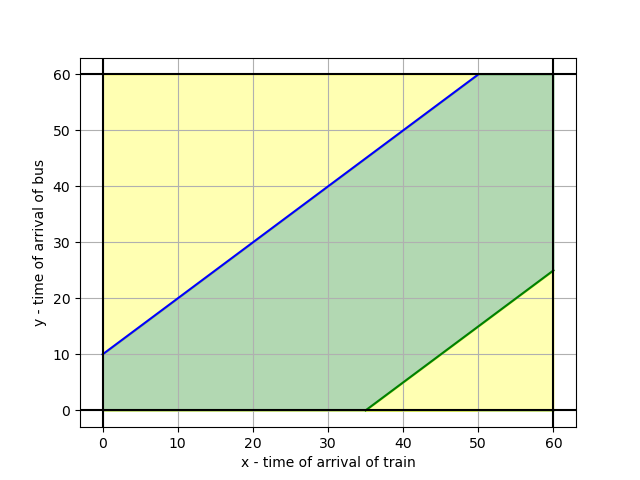
\includegraphics[width = 0.5\textwidth]{graph}
        \caption{Graph between the train and bus timings}
        \label{fig:my_label}
    \end{figure}
\end{frame}
\begin{frame}{Solution}
    Now the points in the green coloured region are our favourable outcomes. Hence the probablility of meeting of bus and train is given by
    \begin{align}
        Probability &= \frac{\text{Area of green region}}{\text{Area of the total region}}
    \end{align}
    We have Probability as  0.5 \newline
    Area of the total region = $60\times 60$ = 3600
\end{frame}

\begin{frame}{Solution}
    \begin{align}
        \text{Area of green region} &= \text{Total Area - area of yellow region} \\
        \text{Area of green region} &= 3600 - \frac{1}{2}(60-10)^2 -\frac{1}{2}(60-k)^2 \\
        &= 3600 - 1250 - \frac{1}{2}(60-k)^2 \\
        &= 2350 - \frac{1}{2}(60-k)^2 \\
        \implies Probability &= \frac{2350 - \frac{1}{2}(60-k)^2}{3600} \\
        0.5 \times 3600 &= 2350 - \frac{1}{2}(60-k)^2\\
        \implies k &= 26.83
    \end{align}
    
\end{frame}

\begin{frame}{Solution}
    Hence the bus must stop for arround 26.83 minutes to meet the train at probability of 0.5
\end{frame}
\end{document}
